\section{Particle-mesh method}
The particle-mesh method can be described as the following sequence of four steps:
\begin{enumerate}
    \item Assign masses to mesh points,
    \item Solve the field equation (\autoref{eq:poisson}) on the mesh,
    \item Calculate the field strength at mesh-points,
    \item Find forces applied to individual particles by interpolation.
\end{enumerate}
In this section, each of these steps will be described in more detail.

\subsection{Mass assignment}\label{subsec:mass-assignment}
The specifics of assigning mass from particles to mesh points depend on the density profile (or \textit{shape}) associated with the particles.
In general, the particles need not be represented as idealized dimensionless points;
indeed, it is possible to construct a hierarchy of shapes, where each successive member covers a larger number of mesh points and whose application leads to smaller numerical errors.

An infinite hierarchy of shapes with this property, as described by Hockney and Eastwood in \cite{Hockney1988}, can be generated by successive convolutions with the ``top-hat'' function $\Pi$, defined as
\begin{equation*}
    \Pi(x) = \begin{cases}
        1,           & |x| < \frac{1}{2} \\
        \frac{1}{2}, & |x| = 1           \\
        0,           & \text{otherwise}.
    \end{cases}
\end{equation*}
The three most popular assignment schemes that hail from this family (and the ones implemented in our program) are the \textit{nearest grid point} (NGP), \textit{cloud in cell} (CIC), and \textit{triangular shaped cloud} (TSC) schemes, with shapes $S$ given by
\begin{align*}
    S_\text{NGP} & = \delta(x), & S_\text{CIC} & = \delta(x) * \frac{1}{H} \Pi\left(\frac{x}{H}\right) = \frac{1}{H}\Pi\left(\frac{x}{H}\right), & S_\text{TSC} & = \frac{1}{H}\Pi\left(\frac{x}{H}\right) * \frac{1}{H}\Pi\left(\frac{x}{H}\right) = \frac{1}{H}\Lambda \left(\frac{x}{H}\right),
\end{align*}
where $\Lambda$ is the triangle function
\begin{equation*}
    \Lambda(x) = \begin{cases}
        1 - |x|, & |x| < 1           \\
        0,       & \text{otherwise}.
    \end{cases}
\end{equation*}
For illustrative purposes, the shape $S_\text{CIC}$ is depicted in \autoref{fig:cic-shape}.
\begin{figure}[htp]
    \centering
    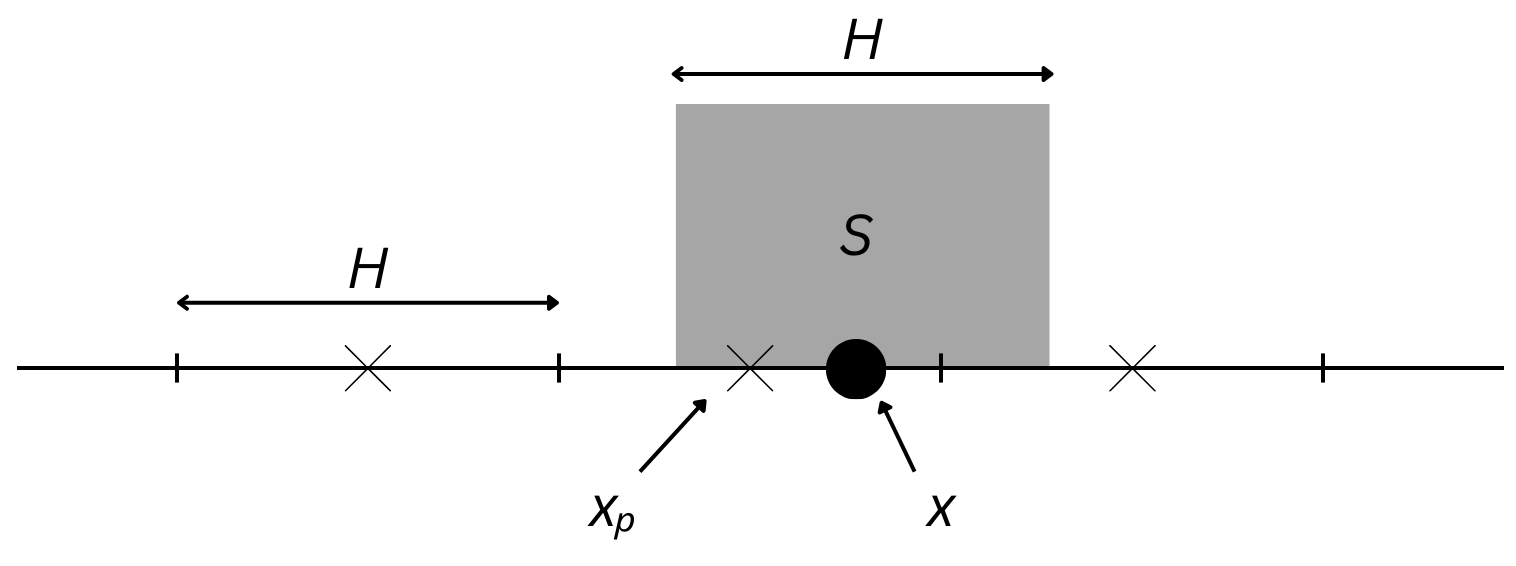
\includegraphics[scale=0.2]{img/CIC.png}
    \caption{The CIC shape centered at $x$ (particle position).
        The particle is within cell $x_p$, however, the cell $x_{p+1}$ gets non-zero density contribution from the particle.}
    \label{fig:cic-shape}
\end{figure}

In the one-dimensional case, the fraction of mass $W_p$ assigned to mesh-point $p$ from particle at position $x$ is given by
\begin{equation*}
    W(x-x_p) = W_p(x) = \int_{x_p-H/2}^{x_p+H/2} S(x'-x)dx'.
\end{equation*}
A simple rule for relating the assignment function $W$ defined above with shape $S$ can be found by noticing that
\begin{equation*}
    W(x) = \int_{-H/2}^{H/2}S(x'-x)dx' = \int_{-\infty}^\infty \Pi\left(\frac{x'}{H}\right)S(x'-x)dx' = \Pi\left(\frac{x}{H}\right) * S(x).
\end{equation*}
This implies that
\begin{align}\label{eq:assignment-functions}
    W_\text{NGP}(x) & = \Pi\left(\frac{x}{H}\right), & W_\text{CIC}(x) & = \Lambda\left(\frac{x}{H}\right), & W_\text{TSC}(x) & = \Pi\left(\frac{x}{H}\right) * \frac{1}{H} \Lambda\left(\frac{x}{H}\right) = (\Pi * \Lambda)\left(\frac{x}{H}\right).
\end{align}
Splitting the domain of integration in the expression for $W_\text{TSC}$ into five disjoint intervals shows that
\begin{equation*}
    (\Pi * \Lambda)(x) = \begin{cases}
        \frac{1}{8}(3-2|x|)^2, & \frac{1}{2} \leq |x| < \frac{3}{2} \\
        \frac{3}{4}-x^2,       & |x| < \frac{1}{2}                  \\
        0,                     & \text{otherwise}.
    \end{cases}
\end{equation*}

Two- and three-dimensional versions of the assignment functions in \autoref{eq:assignment-functions} are products of the assignment functions in each dimension.
For example, the three-dimensional assignment function $W$ is
\begin{equation*}
    W(\mathbf{x}) = W(x)W(y)W(z).
\end{equation*}
Hence, the mass assigned at mesh-point at $\mathbf{x}_\mathbf{p}$ is
\begin{equation*}
    m(\mathbf{x}_\mathbf{p}) = \sum_i m_i W_\mathbf{p}(\mathbf{x}_i),
\end{equation*}
or, in terms of density $\rho$,
\begin{equation}\label{eq:density-assignment}
    \rho(\mathbf{x}_\mathbf{p}) = \frac{1}{V} \sum_i m_i W_\mathbf{p}(\mathbf{x}_i),
\end{equation}
where $V = H^3$ is the volume of a cell and $i$ indexes the particles.

Obviously, \autoref{eq:density-assignment} is not suitable for direct application in the actual algorithm.
Instead, we iterate over all particles, identify the parent cell $\mathbf{p}$ of each particle (and its neighborhood) and update $\rho$.
This process is illustrated in \autoref{alg:density-assignment}.
\begin{algorithm}
    \caption{Density assignment algorithm}\label{alg:density-assignment}
    \begin{algorithmic}[1]
        \ForAll {particle $i$}
        \ForAll {cell $\mathbf{q}$ in $\mathcal{C}_S(\mathbf{x}_i)$}
        \State $\rho(\mathbf{x}_\mathbf{q}) \gets \rho(\mathbf{x}_\mathbf{q}) + m_i W(\mathbf{x}_i - \mathbf{x}_\mathbf{q}) / V$
        \EndFor
        \EndFor
    \end{algorithmic}
\end{algorithm}
The set $\mathcal{C}_S(\mathbf{x}_i)$ of cells that have to be considered while assigning density from the $i$-th particle, depends on the shape $S$ of the particle.
Specifically, we have $\mathcal{C}_\mathrm{NGP}(\mathbf{x}) = \{[\mathbf{x} / H]\}$, $\mathcal{C}_\mathrm{CIC}(\mathbf{x}) = \{\lfloor \mathbf{x}/H \rfloor + \mathbf{t} \;|\; t_i =0,1\}$, and $\mathcal{C}_\mathrm{TSC}(\mathbf{x}) = \{[\mathbf{x} / H] + \mathbf{t} \;|\; t_i = -1, 0, 1\}$.
It follows that $|\mathcal{C}_\mathrm{NGP}(\mathbf{x})| = 1$, $|\mathcal{C}_\mathrm{CIC}(\mathbf{x})| = 8$, and $|\mathcal{C}_\mathrm{TSC}(\mathbf{x})| = 27$ which illustrates the increasing computational cost resulting from using higher-order assignment schemes.
We note that \autoref{alg:density-assignment} can be parallelized if atomic increments are used in line 3.

\subsection{Solving the field equation}
The Poisson equation (\autoref{eq:poisson}) can be restated in integral form
\begin{equation*}
    \phi(\mathbf{x}) = \int \mathcal{G}(\mathbf{x}-\mathbf{x}')\rho(\mathbf{x}') dV',
\end{equation*}
which has the following discrete analogue
\begin{equation}\label{eq:poisson-discrete}
    \phi(\mathbf{x}_\mathbf{p}) = V \sum_{\mathbf{p}'} \mathcal{G}(\mathbf{x}_\mathbf{p} - \mathbf{x}_{\mathbf{p}'}) \rho(\mathbf{x}_{\mathbf{p}'}),
\end{equation}
where $\mathcal{G}$ is the Green's function (potential due to unit mass).
The right-hand side of \autoref{eq:poisson-discrete} is a convolution sum that runs over a finite set of mesh points.
If we assume periodic boundary conditions, we can apply the discrete Fourier transform to both sides and use the convolution theorem to conclude that\footnote{
    In this work, the Hockney \& Eastwood definition of DFT is used, i.e.
    \begin{equation*}
        D(x_p) = \frac{1}{L}\sum_{l=0}^{N-1}\hat{D}(k)e^{ikx_p}, \quad \hat{D}(k) = H\sum_{p=0}^{N-1}D(x_p)e^{-ikx_p},
    \end{equation*}
    where $x_p = pH$.
    The conversion between this form and another popular definition,
    \begin{equation}\label{eq:standard-dft}
        \widetilde{D_H}(k) = \sum_{p=0}^{N-1}D_H(p)e^{-i2\pi kp / N},
    \end{equation}
    is given by
    \begin{equation*}
        \widetilde{D_H}(k) = \frac{1}{H}\hat{D}\left(\frac{2\pi}{NH}k\right),
    \end{equation*}
    where $D_H(p) = pH$.
}
\begin{equation}\label{eq:poisson-fourier-product}
    \hat{\phi}(\mathbf{k}) = \hat{\mathcal{G}}(\mathbf{k}) \hat{\rho}(\mathbf{k}).
\end{equation}

An approximation to $\hat{\mathcal{G}}$ can be found using a discretized version of the Laplacian in \autoref{eq:poisson-discrete}.
Specifically, for a 7-point stencil,
\begin{equation*}
    \begin{split}
        4\pi G\rho(\mathbf{x}_{ijk})
         & =\frac{\phi(\mathbf{x}_{i-1,j,k}) - 2\phi(\mathbf{x}_{ijk})+\phi(\mathbf{x}_{i+1,j,k})}{H^2}   \\
         & + \frac{\phi(\mathbf{x}_{i,j-1,k}) - 2\phi(\mathbf{x}_{ijk})+\phi(\mathbf{x}_{i,j+1,k})}{H^2}  \\
         & + \frac{\phi(\mathbf{x}_{i,j,k-1}) - 2\phi(\mathbf{x}_{ijk})+\phi(\mathbf{x}_{i,j,k+1})}{H^2}.
    \end{split}.
\end{equation*}
Applying the discrete Fourier transform to both sides and using the shift theorem we get
\begin{align*}
    4\pi G \hat{\rho}(\mathbf{k})
     & = \frac{1}{H^2}\sum_{i=1}^{3}\left( e^{-iHk_i} + e^{iHk_i}-2 \right)\hat{\phi}(\mathbf{k})       \\
     & = \frac{1}{H^2} \sum_{i=1}^{3}\left( e^{iHk_i/2} - e^{-iHk_i/2} \right)^2 \hat{\phi}(\mathbf{k}) \\
     & = -\frac{4}{H^2}\sum_{i=1}^{3}\sin^2\left(\frac{Hk_i}{2}\right)\hat{\phi}(\mathbf{k}).
\end{align*}
and hence
\begin{equation*}
    \hat{\phi}(\mathbf{k}) = -4\pi G\underbrace{\frac{(H/2)^2}{\sin^2(Hk_1/2) + \sin^2(Hk_2/2) + \sin^2 (Hk_3/2)}}_{\hat{\mathcal{G}}(\mathbf{k})} \hat{\rho}(\mathbf{k}),
\end{equation*}
where $\hat{\mathcal{G}}$ can be identified by comparison with \autoref{eq:poisson-fourier-product}.
It is worth noting that the constant multiplier $(-4\pi G)$ is often left out of $\hat{\mathcal{G}}$ (this is the convention used in \cite{Hockney1988}).
In the implementation, values of $\hat{\mathcal{G}}$ are computed only once and saved for future look-up.

\subsection{Field strength calculation}
The strength $\mathbf{g}$ of the gravitational field at mesh-point $\mathbf{x}_\mathbf{p}$ can be approximated using a central difference.
Our implementation currently supports two types of finite differences, described below.

The two-point finite difference operator $\mathbf{D}$, whose $x$ component is given by
\begin{equation*}
    D_x(\phi)(\mathbf{x_\mathbf{p}}) = \frac{\phi(\mathbf{x}_{i+1,j,k}) - \phi(\mathbf{x}_{i-1,j,k})}{2H}
\end{equation*}
(and analogously for the $y$ and $z$ components), is second order accurate.

The fourth-order accurate finite difference is given by
\begin{equation*}
    D_x(\phi)(\mathbf{x}_\mathbf{p}) = \alpha\frac{\phi(\mathbf{x}_{i+1,j,k}) - \phi(\mathbf{x}_{i-1,j,k})}{2H} + (1-\alpha)\frac{\phi(\mathbf{x}_{i+2,j,k}) - \phi(\mathbf{x}_{i-2,j,k})}{4H},
\end{equation*}
where $\alpha = 4/3$.

The difference between the accuracy of both methods is illustrated in \autoref{fig:finite-diff-accuracy}.
The figure also provides insight into how the error depends on the value of parameter $\alpha$.
\begin{figure}[htp]
    \centering
    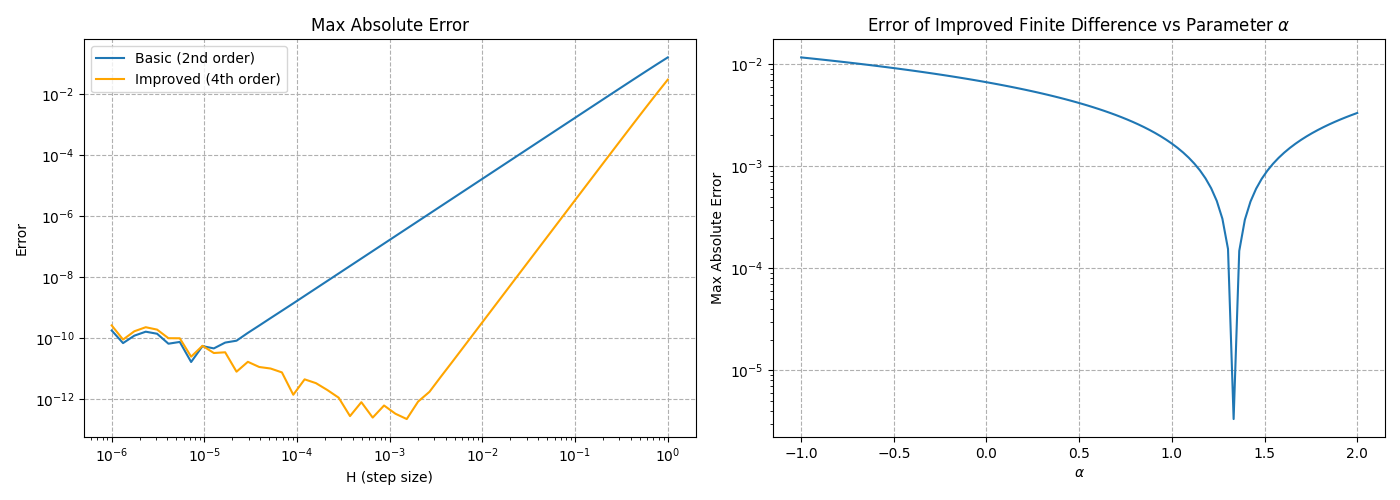
\includegraphics[scale=0.43]{img/finite-diff/finite-difference.png}
    \caption{Left pane: Approximation error for second-order and fourth-order schemes.
        For small values of $H$, round-off errors dominate.
        Right pane: Approximation error vs. $\alpha$ in the improved finite difference scheme ($H = 0.1$).
        Note that the scheme is fourth-order accurate only for $\alpha = 4/3$ (cusp in the graph).}
    \label{fig:finite-diff-accuracy}
\end{figure}

We can alternatively define the finite difference operators in terms of the delta function to get rid of the dependence on the differenced function. (Technically, the resulting quantities are functions rather than operators.)
Consider for example the two-point finite difference in \autoref{eq:two-point-central-diff}.
The definition can be generalized beyond mesh points by letting
\begin{equation*}
    D_j(\phi)(\mathbf{x}) = -\frac{\phi(\mathbf{x} + H \mathbf{e}_j)-\phi (\mathbf{x} - H \mathbf{e}_j)}{2H} = -\int \left[ \frac{\delta(\mathbf{x} + H\mathbf{e}_j - \mathbf{x}') - \delta(\mathbf{x} - H\mathbf{e}_j - \mathbf{x}')}{2H} \right]\phi(\mathbf{x}')d\mathbf{x}',
\end{equation*}
where $\mathbf{e}_j$ is the $j$-th standard basis vector.
This motivates us to define
\begin{equation}\label{eq:two-point-central-diff}
    D_j(\mathbf{x}) = \frac{\delta(\mathbf{x} + H\mathbf{e}_j - \mathbf{x}') - \delta(\mathbf{x} - H\mathbf{e}_j - \mathbf{x}')}{2H}
\end{equation}
and
\begin{equation}\label{eq:four-point-central-diff}
    D_j(\mathbf{x}) = \frac{\delta(\mathbf{x} + H\mathbf{e}_j - \mathbf{x}') - \delta(\mathbf{x} - H\mathbf{e}_j - \mathbf{x}')}{2H} + (1-\alpha)\frac{\delta(\mathbf{x} + 2H\mathbf{e}_j - \mathbf{x}') - \delta(\mathbf{x} - 2H\mathbf{e}_j - \mathbf{x}')}{4H}
\end{equation}
as the two-point as four-point finite difference operators respectively.

If $\phi$ denotes the gravitational potential, then the field $\mathbf{g}$ is approximated at mesh point $\mathbf{x}_\mathbf{p}$ as
\begin{equation*}
    \mathbf{g}(\mathbf{x}_\mathbf{p}) = -\mathbf{D}(\phi)(\mathbf{x}_\mathbf{p}).
\end{equation*}

\subsection{Interpolation}
The value of the field strength $\mathbf{g}(\mathbf{x})$ at the position particle's position $\mathbf{x}$ is calculated by interpolating the values of $\mathbf{g}$ from the neighboring mesh-points.
Formally,
\begin{equation*}
    \mathbf{g}(\mathbf{x}) = \sum_\mathbf{p} W(\mathbf{x} - \mathbf{x}_\mathbf{p}) \mathbf{g}(\mathbf{x}_\mathbf{p}).
\end{equation*}
In practice, there is no need to sum over all mesh points.
Instead, we use an algorithm analogous to \autoref{alg:density-assignment} to only include the cells with non-zero contribution to the sum.
The method is illustrated in \autoref{alg:interpolation}.
\begin{algorithm}
    \caption{Field strength interpolation}\label{alg:interpolation}
    \begin{algorithmic}[1]
        \ForAll {particle $i$}
        \ForAll {cell $\mathbf{q}$ in $\mathcal{C}_S(\mathbf{x}_i)$}
        \State $\mathbf{g}(\mathbf{x}_i) \gets \sum_\mathbf{q} W(\mathbf{x}_i - \mathbf{x}_\mathbf{q}) \mathbf{g}(\mathbf{x}_\mathbf{q})$
        \EndFor
        \EndFor
    \end{algorithmic}
\end{algorithm}
It is important to note that in order to retain correct physical behavior, the interpolation and mass assignment schemes must use the same shape to represent the particles.
The procedure in \autoref{alg:interpolation} is trivially parallelized by converting the sequential loop into a parallel one.

The procedures of density assignment and interpolation presented in \autoref{alg:density-assignment} and \autoref{alg:interpolation} are high level description.
More concrete formulations suitable for direct use in an implementation are given in \cite{Hockney1988} and \cite{Kravtsov2002PM}.

\subsection{Code units}
Implementation of the PM (and \PThreeM{}) methods can be simplified by switching to a system of dimensionless units, often called \textit{code units}.
The natural units of time and length in a PM simulation are $H$ and $DT$, respectively.
Hence, length in a PM code is conveniently expressed in terms of multiples of $H$, and similarly time intervals are given as a multiple of $DT$, i.e. the conversion relations are
\begin{equation*}
    x' = \frac{x}{H} \quad \text{and} \quad t' = \frac{t}{DT}.
\end{equation*}
From there, it follows that
\begin{equation*}
    v' = \frac{DT}{H}v \quad \text{and} \quad a' = \frac{DT^2}{H}a.
\end{equation*}
The expected relation $\mathbf{g}' = -\nabla' \phi'$ leads to the definition $\phi' = (DT^2 / H^2)\phi$.
By stipulating that we have $\nabla'^2\phi = \rho'$, we get $\rho' = DT^2 \cdot 4\pi G\rho$, $m' = (DT^2\cdot 4\pi G / H^3) m$, and $G' = 1/(4\pi)$.

\subsection{Properties of the calculated field}
The field produced by the PM method is neither homogenous nor isotropic.
Anisotropy can be observed by measuring the field generated by a particle in two different directions.
In \autoref{fig:pm-field-properties}, the field strength due to a single source at $x = H$ is shown in two variants: when measured along the $x$-axis (blue line) and the $x=y$ line (orange line).
The difference between these two graphs illustrates anisotropy of the calculated field.
The figure also shows the field strength measured along the $x$-axis when the source was shifted by $H/2$ in the $-x$ direction (green line).
Its deviation from the case when the source was placed at $x=H$ (the blue graph) exemplifies inhomogeneity of the field computed using the PM method.
\begin{figure}[htp]
    \centering
    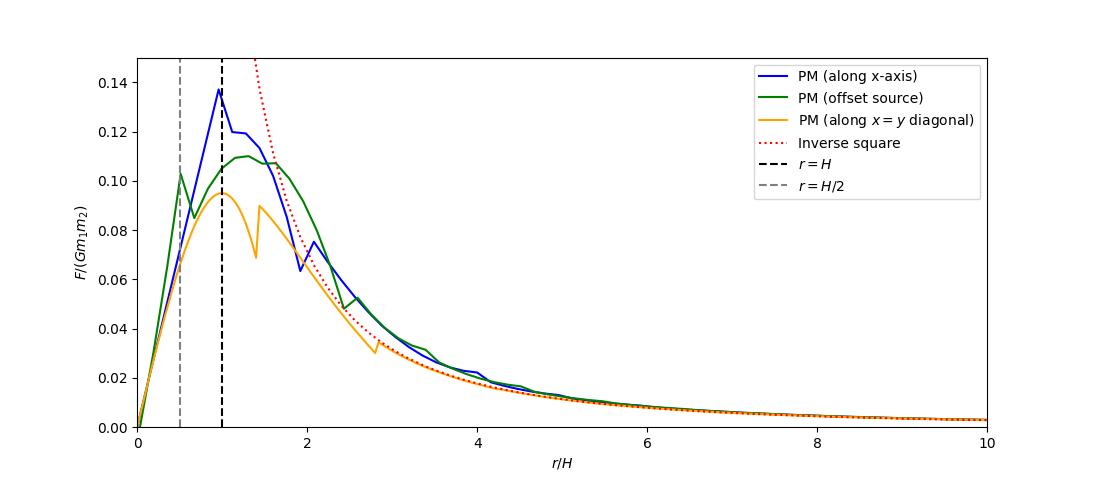
\includegraphics[scale=0.55]{img/pm/pm-field-combined.png}
    \caption{Anisotropy and inhomogeneity of the field as calculated by the PM method (TSC assignment, second order finite difference).}
    \label{fig:pm-field-properties}
\end{figure}
As expected, the PM-calculated approximation gets better with increasing distance from the source;
the inverse-square law is reproduced accurately for $r \gtrsim 4H$.

The single-source case analysis can be extended by considering the effect of choice of finite difference and mass assignment schemes on the relative error between the actual and approximated field strength.
\autoref{fig:pm-combined} shows a comparison of (a) the relative error as a function of distance from the source for PM with second-order and fourth-order finite differences, and (b) the field strength computed using different mass assignment schemes discussed in \autoref{subsec:mass-assignment}.
\begin{figure}[htp]
    \centering
    \begin{subfigure}[t]{0.48\textwidth}
        \centering
        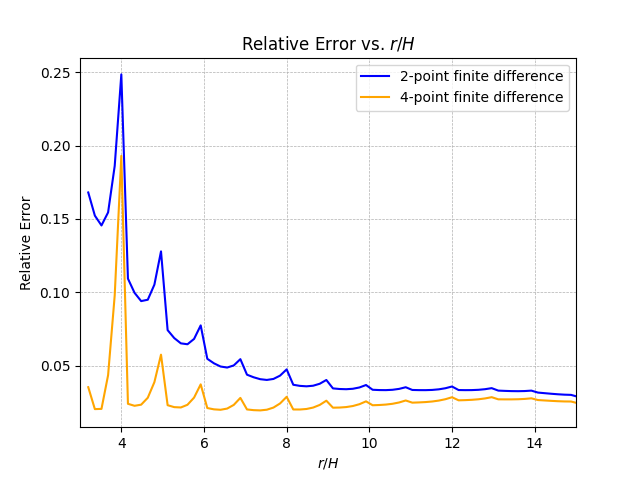
\includegraphics[width=\linewidth]{img/pm/pm-finite-diff-err.png}
        \caption{Relative error of field strength approximation in different PM variants.}
        \label{fig:pm-finite-diff-err}
    \end{subfigure}
    \hfill
    \begin{subfigure}[t]{0.48\textwidth}
        \centering
        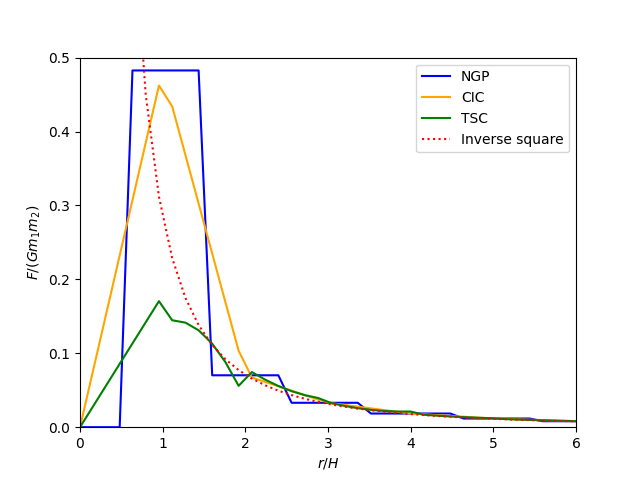
\includegraphics[width=\linewidth]{img/pm/pm-mass-assignment.png}
        \caption{Field strength calculated with the PM method using different assignment schemes.}
        \label{fig:pm-mass-assignment-field-strength}
    \end{subfigure}
    \caption{Comparison of PM method performance. (a) Relative error due to finite difference accuracy. (b) Effect of mass assignment schemes on computed field strength (4-point finite difference).}
    \label{fig:pm-combined}
\end{figure}
The conclusion that can be drawn from \autoref{fig:pm-combined} is that, as expected, the TSC mass assignment scheme and the four-point finite difference yield best results.
